\chapter{}\label{chap4}

\begin{center}
\rule{5cm}{1pt}\\[5pt]
{\Large\bfseries ಸಮಸ್ಯೆಗಳು}\\[3pt]
\rule{5cm}{1pt}
\end{center}

\smallskip
\begin{enumerate}
\renewcommand{\labelenumi}{\bf\theenumi.}
\itemsep=5pt

\item ಹದಿನಾರು 4 ಬಳಸಿ 1000 ಬರಿಸಿ. ಯಾವುದೇ ಗಣಿತೀಯ ಪ್ರಕ್ರಿಯೆ/ಚಿಹ್ನೆ ಬಳಸಬಹುದು.

\item ಯಾವ ಎರಡು ಪೂರ್ಣಾಂಕ ಗುಣಿಸಿದಾಗ 31 ಬರುತ್ತದೆ?

\item 65743 = 26

ಅಂಕಿಗಳ ನಡುವೆ $+$, $-$, $\times$, $()$ ಬಳಸಿ ಸಮೀಕರಣ ಸರಿದೂಗಿಸಿ. ಅಂಕಿಗಳ ಕ್ರಮ ಬದಲಿಸುವಂತಿಲ್ಲ.

\item ಐದು 9 ಬಳಸಿ 10 ಬರಿಸಿ. ಯಾವುದೇ ಗಣಿತ ಪ್ರಕ್ರಿಯೆ ಬಳಸಬಹುದು. 

\item 3 ಪರಸ್ಪರ ಸಮನಾದ ಅಂಕಿ ಬಳಸಿ 24 ಬರಿಸಿ. 8 ಬಳಸಬಾರದು. ಯಾವುದೇ ಗಣಿತ ಪ್ರಕ್ರಿಯೆ (ಘಾತಗಳನ್ನೊಳಗೊಂಡಂತೆ) ಬಳಸಬಹುದು.

\item ಮೂರು 3 ಬಳಸಿ 3 ಬರಿಸಿ. ಯಾವುದೇ ಗಣಿತ ಪ್ರಕ್ರಿಯೆ ಬಳಸಬಹುದು.

\item ಒಂದು ಗೆರೆ ಸ್ಥಾನ ಪಲ್ಲಟ ಮಾಡಿ ಸಮೀಕರನ ಸರಿದೂಗಿಸಿ $\neq$ ಬರುವಂತಿಲ್ಲ. 

VI $-$ II=II

IV=III $-$ I

\item ........do............

\item ಒಂದಕ್ಕೆ 9 ಕೂಡಿಸಿ 20 ಬರಿಸಿ

\item 6 ಬೆಂಕಿಕಡ್ಡಿ  ಬಳಸಿ 100 ಬರಿಸಿ. 

\item ಇವು ಹೇಗೆ ಸಾಧ್ಯ?
\begin{itemize}
\item[(a)] 6 ರ $\frac{2}{3}$~ , ~ 9 ಕ್ಕೆ ಸಮ 
\item[(b)] 5 ರ $\frac{1}{2}$~ , ~ 4 ಕ್ಕೆ ಸಮ
\item[(c)] 11 ರ $\frac{1}{2}$~ , ~ 6 ಕ್ಕೆ ಸಮ
\end{itemize}

\item ಆರರಲಿ ಒಂಭತ್ತು ಕಳೆದು 

ಒಂಭತ್ತರಲಿ ಹತ್ತು ಕಳೆದು 

ನಲವತ್ತರಲಿ ಐವತ್ತು ಕಳೆದರೆ 

ಉಳಿಯುವುದು ಆರು.

ಹೇಗೆ?

\item 8 ಬೆಂಕಿಕಡ್ಡಿಗಳಿವೆ. ಅವುಗಳಲ್ಲಿ ನಾಲ್ಕು ಉಳಿದವುಗಳ ಅರ್ಧದಷ್ಟು ಉದ್ದ. (4 ಕಡ್ಡಿ  2", 4 ಕಡ್ಡಿ 1" ಎಂದು ಭಾವಿಸಿ). ಇವುಗಳನ್ನು ಜೋಡಿಸಿ 3 ಸಮಾನ ಅಳತೆಯ ಚೌಕ ಬರಿಸಿ. 

\item 9 ಬೆಂಕಿಕಡ್ಡಿಗಳಿಂದ 5 ತ್ರಿಭುಜ ರಚಿಸಿ 

\item 4 ಬೆಂಕಿಕಡ್ಡಿ ಬಳಸಿ 1 ಬರಿಸಿ. ಯಾವುದೇ 2 ಕಡ್ಡಿ ಸಮಾಂತರವಾಗಬಾರದು ಅಥವಾ ಒಂದೇ ರೇಖೆಯಲ್ಲಿರಬಾರದು.

\item 9 ಬೆಂಕಿಕಡ್ಡಿ ಜೋಡಿಸಿ, 6 ಚೌಕ ಬರಿಸಿ.

\item 1 ಬೆಂಕಿಕಡ್ಡಿ ಬಾಹುವಿನ 16 ಚೌಕಗಳಿವೆ (4 $\times$ 4)
\begin{itemize}
\item[(a)] ಎಲ್ಲಾ ಅಳತೆಯ ಚೌಕಗಳೆಷ್ಟಿವೆ? 
\item[(b)] ಯಾವುದಾದರೂ 8 ಕಡ್ಡಿ ತೆಗೆದು ಹಾಕಿ ಚೌಕಗಳೆಲ್ಲದಂತೆ ಮಾಡಿ 
\end{itemize}

\item 16 ಬೆಂಕಿಕಡ್ಡಿಗಳಿಂದ ಚೌಕ ರಚಿಸಿದೆ 
\begin{figure}[H]
\centering
\includegraphics{images/chap4/q18.eps}
\end{figure}
\begin{itemize}
\item[(a)] 10 ಕಡ್ಡಿ ಸ್ಥಳಾಂತರಿಸಿ 8 ಸಮಾನ ತ್ರಿಭುಜ ರಚಿಸಿ.
\item[(b)] 7 ಕಡ್ಡಿ ಸ್ಥಳಾಂತರಿಸಿ 5 ನಾಲ್ಕು ಬಾಹು ಆಕೃತಿ ರಚಿಸಿ.
\end{itemize}

\item ಈ ಗುಣಾಕಾರ ಗಮನಿಸಿ.

\begin{tabular}{ccc}
$1 \times 1$ & = & $1$\\
$11 \times 11$ & = & $121$\\
$111 \times 111$ & = & $12321$\\
$1111 \times 1111$ & = & $123421$
\end{tabular}

ಮುಂದಿನ 5 ಹಂತಗಳನ್ನು ಬರೆಯಿರಿ. 

\item ಈ ಗುಣಾಕಾರ ಗಮನಿಸಿ 

\begin{tabular}{rcl}
$9 \times 9 + 7$ & = & $88$\\
$98 \times 9 + 6$ & = & $888$\\
$987 \times 9 + 5$ & = & $8888$
\end{tabular}

ಮುಂದಿನ 5 ಹಂತ ಬರೆಯಿರಿ.

\item 1089 ಒಂದು ವಿಶಿಷ್ಟ ಸಂಖ್ಯೆ. ಇದನ್ನು 1 ರಿಂದ 9 ರವರೆಗೆ ಪ್ರತ್ಯೇಕವಾಗಿ ಗುಣಿಸಿ, ಲಬ್ಧವನ್ನು ಅಡ್ಡಸಾಲಿನಲ್ಲಿ ಒಂದರ ಕೆಳಗೆ ಒಂದರಂತೆ ಬರೆಯಿರಿ. ಕಂಬಸಾಲುಗಳನ್ನು ಗಮನಿಸಿ.

\item ಎರಡಂಕಿಯ ಎರಡು ಸಂಖ್ಯೆಗಳ ಗುಣಲಬ್ಧವು, ಆ ಸಂಖ್ಯೆಗಳನ್ನು ತಿರುವು ಮುರುವು ಮಾಡಿ ಗುಣಿಸಿದಾಗ ಬರುವ ಲಬ್ಧಕ್ಕೆ ಸಮವಾಗಬಹುದು.
\begin{align*}
\text{ಉದಾ:}\quad 12 \times 42 & = 504 = 21 \times 24\\
34 \times 86 & = 2924 = 43 \times 68
\end{align*}

ಇಂತಹ ಮತ್ತೆ ಐದು ಉದಾಹರಣೆ ರಚಿಸಿ.

\item ವೃತ್ತಾಕಾರದ ರೊಟ್ಟಿ ಇದೆ. 5 ಸರಳರೇಖೆಗಳಿಂದ ಕತ್ತರಿಸಿ 13 ಭಾಗ ಬರಿಸಬೇಕು. ಭಾಗಗಳು ಸಮನಾಗಿರಬೇಕಾಗಿಲ್ಲ. ಇನ್ನೂ ಹೆಚ್ಚು ಭಾಗ ಮಾಡಲು ಸಾಧ್ಯವೆ? 

\item ಪ್ಲೇಟೊ ಕನಸಿನಲ್ಲಿ ಒಂದು ಅಮೃತಶಿಲೆಯ ಘನವು ಚೌಕಾಕೃತಿಯ ಅಮೃತಶಿಲೆಯ ಆಧಾರದ ಮಧ್ಯೆ ನಿಂತಿರುವುದನ್ನು ಕಂಡ ಎರಡರಲ್ಲಿಯೂ ಸಮಾನ ಅಳತೆಯ ಚಿಕ್ಕ ಘನಗಳಿದ್ದುವು ಘನದ ಅಳತೆ ಎಷ್ಟು?

\item ಈ ಆಕೃತಿಯಲ್ಲಿರುವ ಎಲ್ಲ ಅಳತೆಯ ತ್ರಿಭುಜಗಳೆಷ್ಟು?

\begin{figure}[H]
\centering
\includegraphics{images/chap4/q25.eps}
\end{figure}

\item ಚಕ್ರ ಕ್ರಾಂಚಾಕುಲಿತ ಸಲಿಲೇ ಕ್ವಾಪಿ ದೃಷ್ಟಂ ಕಟಾಕೇ । 

ಕೋಯಾದೂರ್ಧ್ವಂ ಕಮಲ ಕಲಿಕಾಗ್ರಂ ವಿತಸ್ತಿ ಪ್ರಮಾಣಂ ।।

ಮಂದಂ ಮಂದಂ ಚಲಿತ ಅನಿಲೇನಾಹತಂ ಹಸ್ತಯುಗ್ಮೇ ।

ತಸ್ಮಿನ್ ಮಗ್ನಂ ಗಣಕ ಕಥಯಕ್ಷಿ ಪ್ರಮಂಭ ಪ್ರಮಾಣಂ ।।

\hfill (ಭಾಸ್ಕರಾಚಾರ್ಯರ `ಲೀಲಾವತೀ' ಯಿಂದ)


{\bf ಅರ್ಥ:} ಚಕ್ರ, ಕ್ರಾಂಚ ಪಕ್ಷಿಗಳಿಂದಲೂ ಕಮಲಗಳಿಂದಲೂ ಆವೃತವಾದ ಒಂದು ಕೊಳವಿದೆ. ಅದರಲ್ಲಿ ನೀರಿನ ಮೇಲೆ ಕಾಣುವ ತಾವರೆ ಮೊಗ್ಗು $\dfrac{1}{2}$ ಹಸ್ತ ಪ್ರಮಾಣದಷ್ಟು ಎತ್ತರದಲ್ಲಿದೆ. ನಿಧಾನವಾಗಿ ಬೀಸುವ ಗಾಳಿಯಿಂದ ಮೊಗ್ಗು ಬಾಗಿ 2 ಹಸ್ತ ದೂರದಲ್ಲಿ ಮುಳುಗುತ್ತದೆ. ನೀರಿನ ಆಳವನ್ನು ಬೇಗ ಲೆಕ್ಕ ಹಾಕಿ ಹೇಳು. 

\item ನಾಲ್ಕಂಕಿ ಸಂಖ್ಯೆಯಲ್ಲಿ ಒಂದು ಅಂಕಿ ಹೇಳಿದಾಗ ಉಳಿದ ಮೂರನ್ನು ಹೇಳುವುದು 

ನನಗೆ ಕಾಣದಂತೆ 1 ರಿಂದ 9 ವರೆಗಿನ ಯಾವುದಾದರೂ ಒಂದು ಅಂಕಿ ಬರೆಯಿರಿ 10 ರಿಂದ ಗುಣಿಸಿ. ಮೊದಲ ಅಂಕಿ ಕೂಡಿಸಿ. ಉತ್ತರವನ್ನು 9 ರಿಂದ ಗುಣಿಸಿ. ಲಬ್ಧವನ್ನು 11 ರಿಂದ ಗುಣಿಸಿ. ನಾಲ್ಕಂಕಿ ಸಂಖ್ಯೆ ಬರುತ್ತದೆ. ಅದರ ಬಿಡಿ ಸ್ಥಾನದ (ಏಕ) ಅಂಕಿ ಹೇಳಿ. ಉಳಿದ ಮೂರನ್ನು ನಾನು ಹೇಳುತ್ತೇನೆ.

\item ಬಿಲ್ಲುಗಾರಿಕೆ ಸ್ಪರ್ಧೆಯಲ್ಲಿ ಇಬ್ಬರು ಒಟ್ಟು 800 ಪಾಯಿಂಟ್ಗಳಿಸಿದರು. ಇಬ್ಬರ ಸ್ಕೋರಿನಲ್ಲಿಯೂ ಅದೇ ಮೂರು ಅಂಕಿಗಳಿದ್ದವು ಆದರೆ ಕ್ರಮ ಬೇರೆ. ಅವರ ಸ್ಕೋರುಗಳು ಎಷ್ಟೆಷ್ಟು? 

\item ಒಬ್ಬನಲ್ಲಿ 1023 ಒಂದು ರೂ ನಾಣ್ಯಗಳಿದ್ದವು. ಅವನ್ನು 10 ಚೀಲಗಳಲ್ಲಿ ಬೇರೆ ಬೇರೆ ಸಂಖ್ಯೆಗಳಷ್ಟು ತುಂಬಿಸಿ, ಬಾಯಿಕಟ್ಟಿ, ಚೀಲದ ಮೇಲೆ ಒಳಗಿರುವ ನಾಣ್ಯಗಳ ಸಂಖ್ಯೆ ಬರೆದ. ವಿಶೇಷವೆಂದರೆ ಯಾರು 1 ರಿಂದ 1023ವರೆಗೆ ಕೇಳಿದರೂ ಚೀಲಗಳ ಬಾಯಿ ತೆರೆಯದೆ ಇಡೀ ಚೀಲಗಳನ್ನು ಕೊಡಬಹುದಿತ್ತು. ಹಾಗಾದರೆ ಪ್ರತಿಯೊಂದು ಚೀಲದಲ್ಲಿದ್ದ ನಾಣ್ಯ ಎಷ್ಟು? 

\item ಒಂದು ಸಂಖ್ಯೆಯನ್ನು 3 ರಿಂದ ಗುಣಿಸಿ 1 ನ್ನು ಕೂಡಿಸಿದಾಗ ಒಂದು ಘನ ಸಂಖ್ಯೆ ಬರುತ್ತದೆ. ಘನ ಸಂಖ್ಯೆಯ ಘನ ಮೂಲ ವರ್ಗವನ್ನು 3 ರಿಂದ ಗುಣಿಸಿ 1 ನ್ನು ಕೂಡಿಸಿದಾಗ ಒಂದು ವರ್ಗ ಸಂಖ್ಯೆ ಲಭಿಸುತ್ತದೆ. ಸಂಖ್ಯೆ ಯಾವುದು?
\end{enumerate}

\smallskip

\begin{center}
\rule{5cm}{1pt}\\[3pt]
{\Large\bfseries ಉತ್ತರಗಳು}\\[-0.1cm]
\rule{5cm}{1pt}
\end{center}

\begin{enumerate}
\item $\underbrace{444 + 444}_{888} + \underbrace{44 + 44}_{88} + \underbrace{4 + 4 + 4 + 4 + 4 + 4}_{24}$

$888 + 88 + 24 = 1000$

\item $31 \times 1 = 31$

\item $(6- 5) + (7 \times 4) - 3 = 26$

\item $9 + \dfrac{99}{99} = 9 + 1 = 10$

\item $3^{3} - 3 = 27 - 3 = 24$

\item $3 + 3 - 3 = 3$; $3 \times \dfrac{3}{3} = 3$; $\sqrt[3]{3^{3}} = 3$

\item V $-$ III = II\quad (VI ನ 1 ಗೆರಯನ್ನು II ಗೆ ಸೇರಿಸಿದೆ)

IV $-$ II = II\quad (IV ನ 1 ಗೆರಯನ್ನು  V ಹಿಂಬದಿ ಬರೆದಿದೆ)

\item IV $-$ III = I\quad ($=$ ನ ಒಂದು ಅಡ್ಡ ಗೆರೆಯನ್ನು $-$ ಮೇಲೆ ಬರೆದಿದೆ)

\item 9 ಎಂದರೆ IX ; (IX + 1) XX (1 ರಿಂದ IXನ 1ನ್ನು ಹೊಡೆದಿದೆ)

\item 
\begin{figure}[H]
\centering
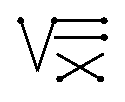
\includegraphics{images/chap4/ans10.eps}
 = $\sqrt{10,000} = 100$
\end{figure}

($\overline{X} = 10,000$)

\item 
\begin{itemize}
\item[(a)] $6 - 51x$ ಮೂರಕ್ಷರದಲ್ಲಿ S ಬಿಡಿ $\dfrac{2}{3}$ ಭಾಗ ಉಳಿದಿದೆ. 
\item[(b)] $5 -$ FIVE : F ಮತ್ತು E ಬಿಡಿ $\dfrac{1}{2}$ ಭಾಗ ಉಳಿದಿದೆ  IV = 4
\item[(c)] II ನ್ನು ರೋಮನ್ ಅಂಕಿಯಲ್ಲಿ ಬರೆಯಿರಿ XI ಅಡ್ಡಲಾಗಿ ಕತ್ತರಿಸಿ XI ಉಳಿಯುವುದು ಮೇಲ್ಭಾಗ VI = 6
\end{itemize}

\item 
\begin{equation*}
\begin{tabular}[t]{r}
51X \\
1X\\\cline{1-1} 
Xl
\end{tabular}
\quad
\begin{tabular}[t]{r}
1X\\ 
X\\\cline{1-1} 
1
\end{tabular}
\quad
\begin{tabular}[t]{r}
5\\
1\\\cline{1-1}
X
\end{tabular}
\end{equation*}

ಉಳಿದಿರುವುದು 51X ಆರು (6)

\item 1, 2, 3, 4 ಅರ್ಧ ಉದ್ದ ಉಳಿದ ನಾಲ್ಕು ಪೂರ್ಣ ಉದ್ದ

\begin{figure}[H]
\centering
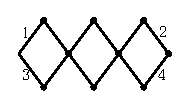
\includegraphics{images/chap4/ans13.eps}
\end{figure}

\item 4 ಸಮಬಾಹು ತ್ರಿಭುಜಗಳು ಚಿಕ್ಕವು 1 ದೊಡ್ಡ ತ್ರಿಭುಜ

\begin{figure}[H]
\centering
\includegraphics{images/chap4/ans14.eps}
\end{figure}

\item
\begin{figure}[H]
\centering
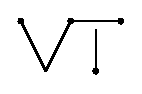
\includegraphics{images/chap4/ans15.eps}
 = 1
 \end{figure}

\item 
\begin{figure}[H]
\centering
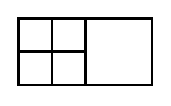
\includegraphics{images/chap4/ans16.eps}
 \end{figure}

\item 
\begin{itemize}
\item[(a)] $1^{2} + 2^{2} + 3^{2} + 4^{2} = 1 + 4 + 9 + 16 = 30$ ಚೌಕಗಳು 
\item[(b)] 23, 5, 9, 10, 11, 13, 16, 19 ತೆಗೆದಿದೆ.
\end{itemize}

\begin{figure}[H]
\centering
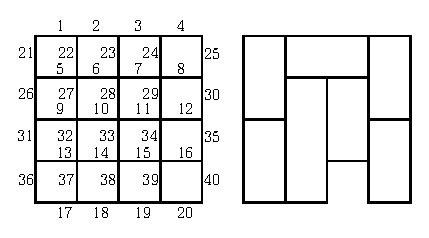
\includegraphics{images/chap4/ans17.eps}
\end{figure}

\item 
\begin{figure}[H]
\centering
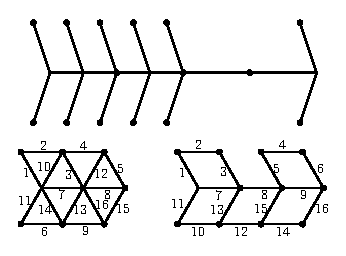
\includegraphics{images/chap4/ans18.eps}
\end{figure}

\item 

\smallskip
\begin{tabular}[t]{ccr}
$11111 \times 11111$ & = & $123454321$\\
$111111 \times 111111$ & = & $12345654321$\\
$1111111 \times 1111111$ & = & $1234567654321$\\
$11111111 \times 11111111$ & = & $123456787654321$\\
$111111111 \times 111111111$ & = & $1234567897654321$\\
\end{tabular}

\item 

\smallskip
\begin{tabular}[t]{ccr}
$9876 \times 9 + 4$ & = & $88888$\\
$98765 \times 9 + 3$ & = & $888888$\\
$987654 \times 9 + 2$ & = & $8888888$\\
$9876543 \times 9 + 1$& = & $88888888$\\
$98765432 \times 9 + 0$ & = & $888888888$
\end{tabular}

\item 

\smallskip
\begin{tabular}[t]{ccccccc}
$1089 \times 1$ & = & $1$&$0$&$8$&$9$\\
$1089 \times 2$ & = & $2$&$1$&$7$&$9$\\
$1089 \times 3$ & = & $3$&$2$&$6$&$7$\\
$1089 \times 4$ & = & $4$&$3$&$5$&$6$\\
$1089 \times 5$ & = & $5$&$4$&$4$&$5$\\
$1089 \times 6$ & = & $6$&$5$&$3$&$4$\\
$1089 \times 7$ & = & $7$&$6$&$2$&$3$\\
$1089 \times 8$ & = & $8$&$7$&$1$&$2$\\
$1089 \times 9$ & = & $9$&$8$&$0$&$1$
%& & $\downarrow$&$\uparrow$&$\downarrow$&$\uparrow $
\end{tabular}

ಬಾಣದ ಗುರುತಿನ ನೇರದಲ್ಲಿ ಅಂಕಿಗಳು ಕ್ರಮಾಗತವಾಗಿದೆ. 

\item 
\begin{tabular}[t]{ccccc}
$24 \times 63$ & = & $1512$ & = & $42 \times 36$\\
$13 \times 62$ & = & $806$ & = & $31 \times 26$\\
$36 \times 84$ & = & $3024$ & = & $63 \times 48$\\
$46 \times 96$ & = & $4416$ & = & $64 \times 69$\\
$26 \times 93$ & = & $2419$ & = & $62 \times 39$\\
\end{tabular}

\item 
\begin{figure}[H]
\centering
\includegraphics{images/chap4/ans23a.eps}
\includegraphics{images/chap4/ans23b.eps}
\end{figure}

\item ಯಾವುದೇ ವರ್ಗ ಸಂಖ್ಯೆಯ ಅನವು ಮತ್ತೊಂದು ವರ್ಗ ಸಂಖ್ಯೆಯಾಗಬೇಕು 
\begin{align*}
4\text{ ನ್ನು ಪರಿಶೀಲಿಸಿ} \quad 4\times4\times4 & = 64\\
64 &= 8^{2}
\end{align*}

$\therefore$~ ಘನದ ಅಂಚು 4ಮಾನ\quad ಆಧಾರದ ಅಂಚು 8ಮಾನ

\item 35 ತ್ರಿಭುಜಗಳು

\begin{tabular}[t]{ccccc}
ABC & ASC & CRQ & & \\
ABD & AQD & CQD & &\\
ABE & BCD & CRD & &\\
APB & BPQ & CBD & &\\
AQB & BRC & DRE & &\\
APT & BAT & DSE & &\\
ATE & BPC & DTE & &\\
ADC & BQC & DQA & &\\
AED & CDE & DTB & ETS  & EPA\\
AEC & CPE & DSR & ESA  &\\
& & DEB & EST  &\\
\end{tabular}

\begin{figure}[H]
\centering
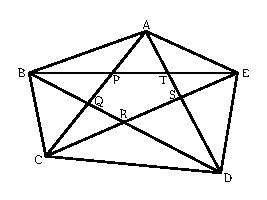
\includegraphics{images/chap4/ans25.eps}
\end{figure}

\item  
\begin{figure}[H]
\centering
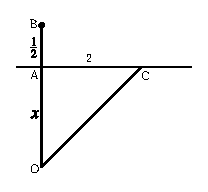
\includegraphics{images/chap4/ans26.eps}
\end{figure}

OB ಕಮಲದ ದಂಟಿರಲಿ 

AC ನೀರಿನ ಮೇಲ್ಮೈ 

B ತಾವರೆಯ ಮೊಗ್ಗು 

C ಮೊಗ್ಗು ಮುಳುಗಡೆ ಸ್ಥಳ 

AB = $\dfrac{1}{2}$ ಹಸ್ತ,\quad AC = 2 ಹಸ್ತ

AO = $x$\quad ಇರಲಿ\quad OB = OC

OAC ಲಂಬಕೋನ ತ್ರಿಭುಜ 
\begin{align*}
\therefore~ OC^{2} & = OA^{2} + AC^{2}\\
\left(x + \dfrac{1}{2}\right)^{2} & = x^{2} + 2^{2} \qquad(\therefore~ OB = OC)\\
x^{2} + x + \dfrac{1}{4} & = x^{2} + 2^{2}\\
x & = 4 - \dfrac{1}{4} = 3\dfrac{3}{4} \quad\text{ ಹಸ್ತ}
\end{align*}

\item  ಉದಾ: ಅವರು 3ನ್ನು ಇಟ್ಟು ಕೊಳ್ಳಲಿ 

$3 \times 10 = 30$~;~~$30 + 3 = 33$~;~~$33 \times 9 = 297$~;~~$297 \times 11 = 3267$ 

ಏಕಸ್ಥಾನದ ಅಂಕಿ 7 ಎಂದು ಹೇಳುತ್ತಾರೆ 

\begin{tabular}{l}
$10$ ರ ಸ್ಥಾನದ ಅಂಕಿ $7-1 = 6$\\
$100$ ರ ಸ್ಥಾನದ ಅಂಕಿ $9-7 = 2$\\
$1000$ ರ ಸ್ಥಾನದ ಅಂಕಿ $9-6 = 3$
\end{tabular}

\item $436$ ಮತ್ತು $364$ (ಒಟ್ಟು $800$)

\item ಅವನು ತುಂಬಿಸಿದ್ದು: 1, 2, 4, 8, 16, 32, 64, 128, 256, 512

ಇದು $2^{0}, 2^{1}, 2^{2}, 2^{3}, 2^{4}, 2^{5}, 2^{6}, 2^{7}, 2^{8}, 2^{9}$ ಶ್ರೇಣಿಯಾಗುತ್ತದೆ 

ಉದಾ: 127 ರೂ ಬೇಕಾದರೆ - $64+32+16+8+4+2+1$

543 ರೂ ಬೇಕಾದರೆ $512+32+2+1$

\item ಸಂಖ್ಯೆ 21
\begin{gather*}
21 \times 3=63;\quad 63+1=64;\quad 64=4^{3}\\
4^{2}=16;\quad 16\times 3=48;\quad 48+1=49=7^{2}
\end{gather*}
\end{enumerate}
